% Slide bodies of dsbm_appendix.tex. Numbers: docs/flow/dsbm/*.csv; tables/*.tex
% are written by scripts/flow/dsbm_tables.py.

% ---------------------------------------------------------------- A1
\begin{frame}{Appendix: a learned Schr\"odinger-bridge coupling on the closure test}
\small
\textbf{Question.} Minibatch OT-CFM loses each jet's fine structure in the known-modification closure
test ($T(J) = 0.8\,[0.8J + 0.2K(J)]$, parent-disjoint unpaired pools): it pairs each jet with another
real jet. Does an online bridge whose training endpoints are \emph{generated by the model} do better?
This tests the Schr\"odinger-bridge (SB) coupling of $\|x - y\|^2/2$ at noise $\varepsilon$ in the model
coordinates, not whether marginal matching finds the physical modification.

\vspace{0.2em}
\begin{columns}[T]
\column{0.52\textwidth}
\footnotesize
\textbf{Online \dsbm{}} (De Bortoli et al.\ 2024, Alg.\ 1)
\begin{itemize}\setlength\itemsep{0.02em}
\item one UVCGAN-S net (32.8M) for both drifts; inputs: state, time, direction
\item bridge $x_t = (1-t)x_0 + t x_1 + \sqrt{\varepsilon t(1-t)}\,z$; the same $\varepsilon$ in the
  Euler-Maruyama sampler (30 steps); Appendix J endpoint preconditioning
\item stage 1: bridge matching on independent real pairs; stage 2: EMA rollouts without gradient,
  real $X_0 \to \hat X_1$ trains the backward drift, real $X_1 \to \hat X_0$ the forward one
\item no true pairs, OT, adversarial or shape losses, teacher
\item $\varepsilon = 1$ fixed before scoring (midpoint noise 0.5 in $z$); $\varepsilon = 0.25$ run only
  because $\varepsilon = 1$ failed with its error dominated by sampling spread (pre-registered)
\end{itemize}
\column{0.48\textwidth}
\footnotesize
\textbf{Arms} (seed 0, one A6000 each, GPU hours incl.\ rollouts)
\begin{itemize}\setlength\itemsep{0.02em}
\item \br{} pretrained 0.5 h; \dsbm{}: 0.5 + 1.5 h refinement; \br{} continued: 0.5 + 1.5 h of
  independent-pair training (the matched control)
\item \ot{} with the same backbone: 2 h, exact minibatch OT, $L^2$
\item $^\dagger$ historical U-Net references (ODE): \pai{} control, OT-CFM
\end{itemize}
\textbf{Gaussian check first} (same code, analytic SB answer): refinement reaches the SB coupling
within 1-3\% with a drift linear in $x$; the paper's MLP overshoots 3-7\%; the pretrained-only sampler
(12\% short) and a wrong-sign coupling fail.
\end{columns}
\end{frame}

% ---------------------------------------------------------------- A2
\begin{frame}{Result: better than not learning the coupling, still 2.4-3$\times$ the identity}
\vspace{-0.5em}
\begin{center}
\scriptsize
\setlength{\tabcolsep}{3pt}
\begin{tabular}{lrrrrrrrr}
\toprule
 & \multicolumn{4}{c}{shape EMD to $T(J)$} & EMD & $E_{out}/E_{in}$ & $E$ RMSE & towers $>$5 GeV \\
 & mean & median & p90 & p99 & GeV & (0.8) & GeV & mean/rms, GeV \\
\midrule
identity $F(J) = J$ & 0.0322 & 0.0317 & 0.039 & 0.047 & 7.03 & 1.000$\pm$0.000 & 6.61 & 4.05 / 4.45 \\
\pai{} control$^\dagger$ & 0.0002 & 0.0001 & 0.000 & 0.000 & 0.02 & 0.800$\pm$0.000 & 0.02 & -0.01 / 0.01 \\
\ot{} U-Net, $L^2$$^\dagger$ & 0.0896 & 0.0768 & 0.151 & 0.274 & 3.56 & 0.785$\pm$0.079 & 2.83 & -1.82 / 3.44 \\
\ot{} U-Net, shape+$E$$^\dagger$ & 0.0914 & 0.0825 & 0.143 & 0.240 & 2.87 & 0.808$\pm$0.037 & 1.32 & -0.87 / 2.16 \\
\ot{} U-Net, s+$E$, pool 1024$^\dagger$ & 0.0760 & 0.0695 & 0.116 & 0.188 & 2.37 & 0.802$\pm$0.032 & 1.10 & -0.50 / 1.61 \\
\ot{} UVCGAN, $L^2$ & 0.0915 & 0.0791 & 0.152 & 0.284 & 4.02 & 0.778$\pm$0.102 & 3.65 & -1.49 / 3.60 \\
\br{} pretrained, $\varepsilon$ 1 & 0.1940 & 0.1507 & 0.360 & 0.731 & 7.62 & 0.799$\pm$0.169 & 5.49 & -2.97 / 5.36 \\
\br{} continued, $\varepsilon$ 1 & 0.1953 & 0.1520 & 0.363 & 0.729 & 7.56 & 0.788$\pm$0.164 & 5.38 & -3.11 / 5.35 \\
\dsbm{}, $\varepsilon$ 1 & 0.0966 & 0.0901 & 0.142 & 0.224 & 5.75 & 0.818$\pm$0.170 & 5.49 & -1.45 / 4.18 \\
\br{} pretrained, $\varepsilon$ 0.25 & 0.2053 & 0.1582 & 0.408 & 0.718 & 7.47 & 0.782$\pm$0.153 & 5.12 & -2.84 / 5.01 \\
\br{} continued, $\varepsilon$ 0.25 & 0.2172 & 0.1649 & 0.445 & 0.757 & 7.53 & 0.781$\pm$0.145 & 4.82 & -3.07 / 5.19 \\
\dsbm{}, $\varepsilon$ 0.25 & 0.0771 & 0.0678 & 0.124 & 0.237 & 4.42 & 0.796$\pm$0.129 & 4.34 & -0.44 / 3.38 \\
\bottomrule
\end{tabular}

\end{center}
\vspace{-0.4em}
\snote{20k held-out test pairs, one output per jet (bridges: one SDE sample, 30 steps, fixed seed; OT-CFM:
ODE, 32 NFE); checkpoints selected on validation only. $^\dagger$ historical U-Net runs (ODE).}

\vspace{0.2em}
\footnotesize
\textbf{Pre-registered gate: fails at both noise levels.} $\varepsilon = 1$: not below OT-CFM with the same
backbone (0.097 vs 0.092) and 3$\times$ the identity. $\varepsilon = 0.25$: 16\% below that OT-CFM and a
better hard core ($-0.44$ vs $-1.49$ GeV), but 2.4$\times$ the identity and worse distributions (mass
W1/$\sigma$ 0.35 vs 0.12; mass change 1.38$\times$ the truth, girth change 0.10$\times$).
\textbf{Measured:} at equal GPU hours the online refinement halves the error of continued independent-pair
training (0.097 vs 0.195; 0.077 vs 0.217).
\end{frame}

% ---------------------------------------------------------------- A3
\begin{frame}{Why: at $\varepsilon = 1$ the sampling spread dominates; at $\varepsilon = 0.25$ a systematic error}
\vspace{-0.9em}
\begin{center}
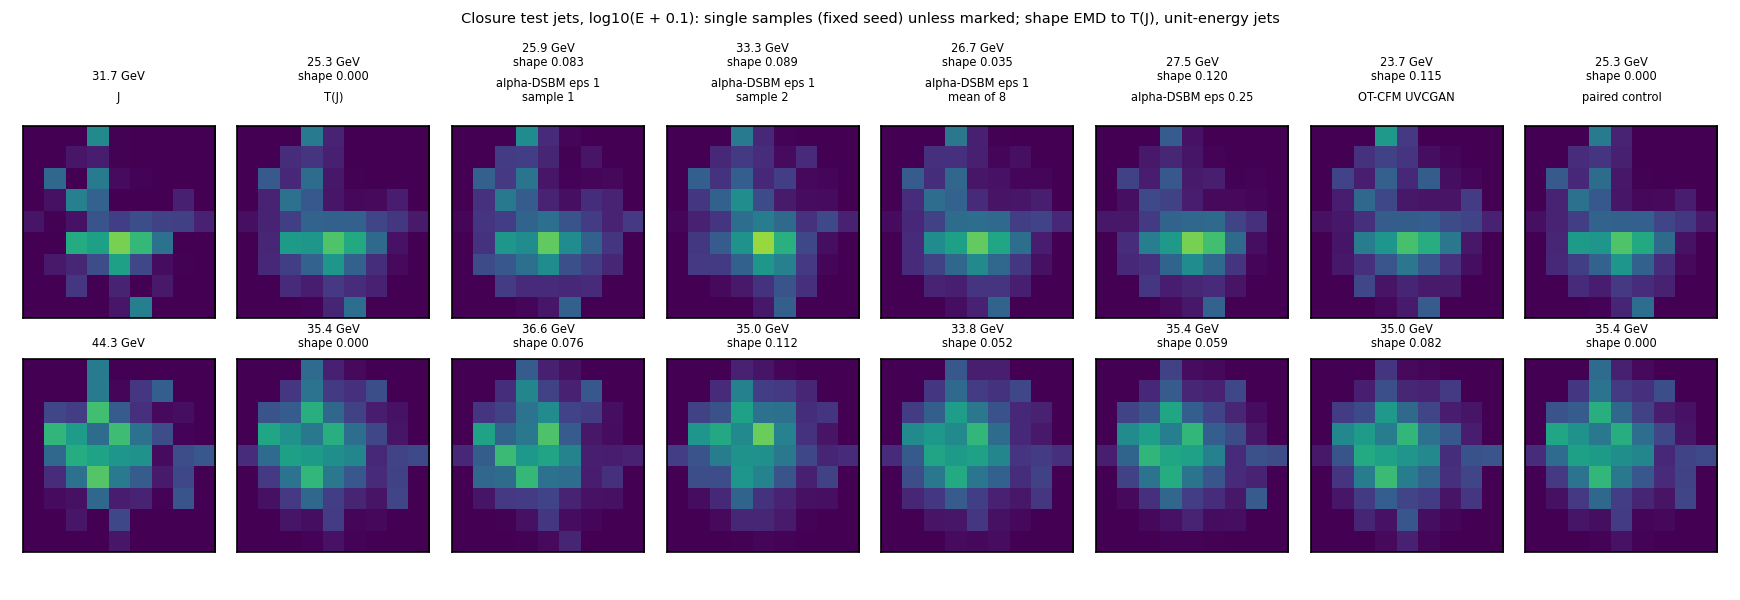
\includegraphics[width=0.8\textwidth]{closure_test_jets_slide.png}
\end{center}
\vspace{-1.3em}
\begin{center}
\scriptsize
\setlength{\tabcolsep}{3pt}
\begin{tabular}{lrrrrrrr}
\toprule
 & \multicolumn{3}{c}{val, 1000 jets: shape EMD} & \multicolumn{4}{c}{test, 1000 jets, 8 samples each} \\
 & to $T(J)$ & 2 samples & 30 vs 60 steps & one sample & 2 samples & mean image & spread $E/\sigma_E$ \\
\midrule
\br{} pretrained, $\varepsilon$ 1 & 0.192 & 0.222 & 0.016 & 0.191 & 0.220 & 0.130 & 0.706 \\
\br{} continued, $\varepsilon$ 1 & 0.193 & 0.224 & 0.015 & 0.192 & 0.221 & 0.132 & 0.669 \\
\dsbm{}, $\varepsilon$ 1 & 0.099 & 0.116 & 0.013 & 0.096 & 0.118 & 0.057 & 0.700 \\
\br{} pretrained, $\varepsilon$ 0.25 & 0.201 & 0.195 & 0.012 & 0.200 & 0.191 & 0.158 & 0.531 \\
\br{} continued, $\varepsilon$ 0.25 & 0.211 & 0.209 & 0.015 & 0.212 & 0.204 & 0.167 & 0.507 \\
\dsbm{}, $\varepsilon$ 0.25 & 0.079 & 0.062 & 0.006 & 0.077 & 0.064 & 0.064 & 0.449 \\
\bottomrule
\end{tabular}

\end{center}
\vspace{-0.6em}
{\scriptsize $\varepsilon = 1$: two samples of a jet differ more than either differs from $T(J)$; a jet's
energy varies by 70\% of the population spread. $\varepsilon = 0.25$: the spread halves and the mean of 8
samples is barely better than one: the error is systematic. 30 steps resolve the SDE.}
\end{frame}

% ---------------------------------------------------------------- A4
\begin{frame}{Cost, and what this does and does not show}
\vspace{-0.6em}
\begin{center}
\scriptsize
\setlength{\tabcolsep}{3pt}
\begin{tabular}{lrrrrrrr}
\toprule
 & GPU h & updates & updates/s & peak GB & selected at & NFE & ms / jet \\
\midrule
\pai{} control$^\dagger$ & 2.00 & 89.8k & 12.5 & 2.9 & 2.00 h & 32 & 2.97 \\
\ot{} U-Net, $L^2$$^\dagger$ & 2.00 & 84.0k & 11.7 & 3.0 & 1.33 h & 32 & 2.96 \\
\ot{} U-Net, shape+$E$$^\dagger$ & 2.00 & 81.5k & 11.3 & 3.0 & 1.83 h & 32 & 2.96 \\
\ot{} U-Net, s+$E$, pool 1024$^\dagger$ & 2.00 & 17.2k & 2.4 & 3.0 & 2.00 h & 32 & 2.96 \\
\ot{} UVCGAN, $L^2$ & 2.00 & 122.8k & 17.1 & 3.5 & 1.67 h & 32 & 1.62 \\
\br{} pretrained, $\varepsilon$ 1 & 0.50 & 26.9k & 14.9 & 3.6 & 0.50 h & 30 & 1.53 \\
\br{} continued, $\varepsilon$ 1 & 2.00 & 107.5k & 14.9 & 3.8 & 1.67 h & 30 & 1.53 \\
\dsbm{}, $\varepsilon$ 1 & 2.00 & 35.9k & 1.7 & 3.8 & 2.00 h & 30 & 1.53 \\
\br{} pretrained, $\varepsilon$ 0.25 & 0.50 & 27.0k & 15.0 & 3.6 & 0.17 h & 30 & 1.53 \\
\br{} continued, $\varepsilon$ 0.25 & 2.00 & 108.2k & 15.0 & 3.8 & 1.50 h & 30 & 1.53 \\
\dsbm{}, $\varepsilon$ 0.25 & 2.00 & 35.8k & 1.6 & 3.8 & 2.00 h & 30 & 1.53 \\
\bottomrule
\end{tabular}

\end{center}
\vspace{-0.5em}
\snote{One A6000 each. GPU h: pretraining and rollouts included; updates: all stages; updates/s: the last stage
(\dsbm{} spends 89\% of its refinement in rollouts, 7680 NFE per update). Latency: batch 2000.}

\vspace{0.1em}
\scriptsize
\begin{columns}[T]
\column{0.5\textwidth}
\textbf{Measured}
\begin{itemize}\setlength\itemsep{0.0em}
\item the code reaches the analytic SB coupling when the network can represent it (Gaussian check)
\item online refinement moves the coupling far from the independent-pair bridge at equal cost
\item neither noise level approaches the identity's per-jet accuracy; $\varepsilon = 0.25$ was still improving
  at 2 GPU h (its limit is open, the gate is not: 0.077 vs 0.032)
\end{itemize}
\column{0.5\textwidth}
\textbf{Not shown}
\begin{itemize}\setlength\itemsep{0.0em}
\item algorithmic success is not the physical correspondence: the SB coupling of $\|x - y\|^2$ in
  $\log E$ is a choice, and $T$ is not its answer
\item robustness: one seed; no second seed or M $\to$ B pilot (gate failed)
\item why $\varepsilon = 0.25$ distorts mass and girth (error amplification in the online loop, as for
  the Gaussian MLP, is a hypothesis)
\end{itemize}
\end{columns}
\end{frame}
